% Template pour poster.

\documentclass{beamer}
\usepackage[T1]{fontenc}
\usepackage[utf8]{inputenc}

\usepackage{array}
\usepackage{amstext}
\usepackage{graphicx}
\makeatletter
\usepackage{multirow}
\usepackage{color}
\usepackage{exscale}
\usepackage{pifont}
\usepackage{xspace}
\usepackage{array}
\usepackage{subfigure}
\usepackage[backend=biber,style=alphabetic]{biblatex}

% NOTE: le paramètre scale permet d'augmenter la taille des polices partout 
% dans le document
\usepackage[orientation=portrait, size=a0, scale=1.1]{beamerposter}

\usetheme{olibposter}

% Set colors for blocks (without frame)
\setbeamercolor{block title}{fg=dblue,bg=white}
\setbeamercolor{block body}{fg=black,bg=white}
\setbeamercolor{block alerted title}{fg=white,bg=dblue!70}%frame color
\setbeamercolor{block alerted body}{fg=black,bg=dblue!10}%body color

% Titre, date, auteurs
\title{SLDC: an open-source workflow for object detection in multi-gigapixels images}
\author{Romain Mormont, Jean-Michel Begon, Renaud Hoyoux, Raphaël Marée\\
{\tt r.mormont@student.ulg.ac.be, jm.begon@ulg.ac.be, renaud.hoyoux@ulg.ac.be, raphael.maree@ulg.ac.be}}
\institute{Systems and modeling, Department of EE \& CS, University of Liège, Belgium}
\date{Année académique 2013-2014}

%% Add bibliography database
\addbibresource{bibliography.bib}

\begin{document}
\begin{frame}

\vspace*{-1cm}
\begin{columns}[t]

\column{.45\paperwidth}


\begin{block}{Object detection and classification}	
\begin{itemize}
\item In some fields of applications, \textbf{multi-gigapixel images} must analysed to gather information and take decision.
\item The analysis usually consist in \textbf{finding some objects} in the images and to associate them with a field-related labels.
\item In cytology, cytopathologists analyze microscope slides in order to find malignant cells or artefacts to \textbf{diagnose diseases like cancer} (see Figure below).
\end{itemize}

\begin{figure}[H]
\center
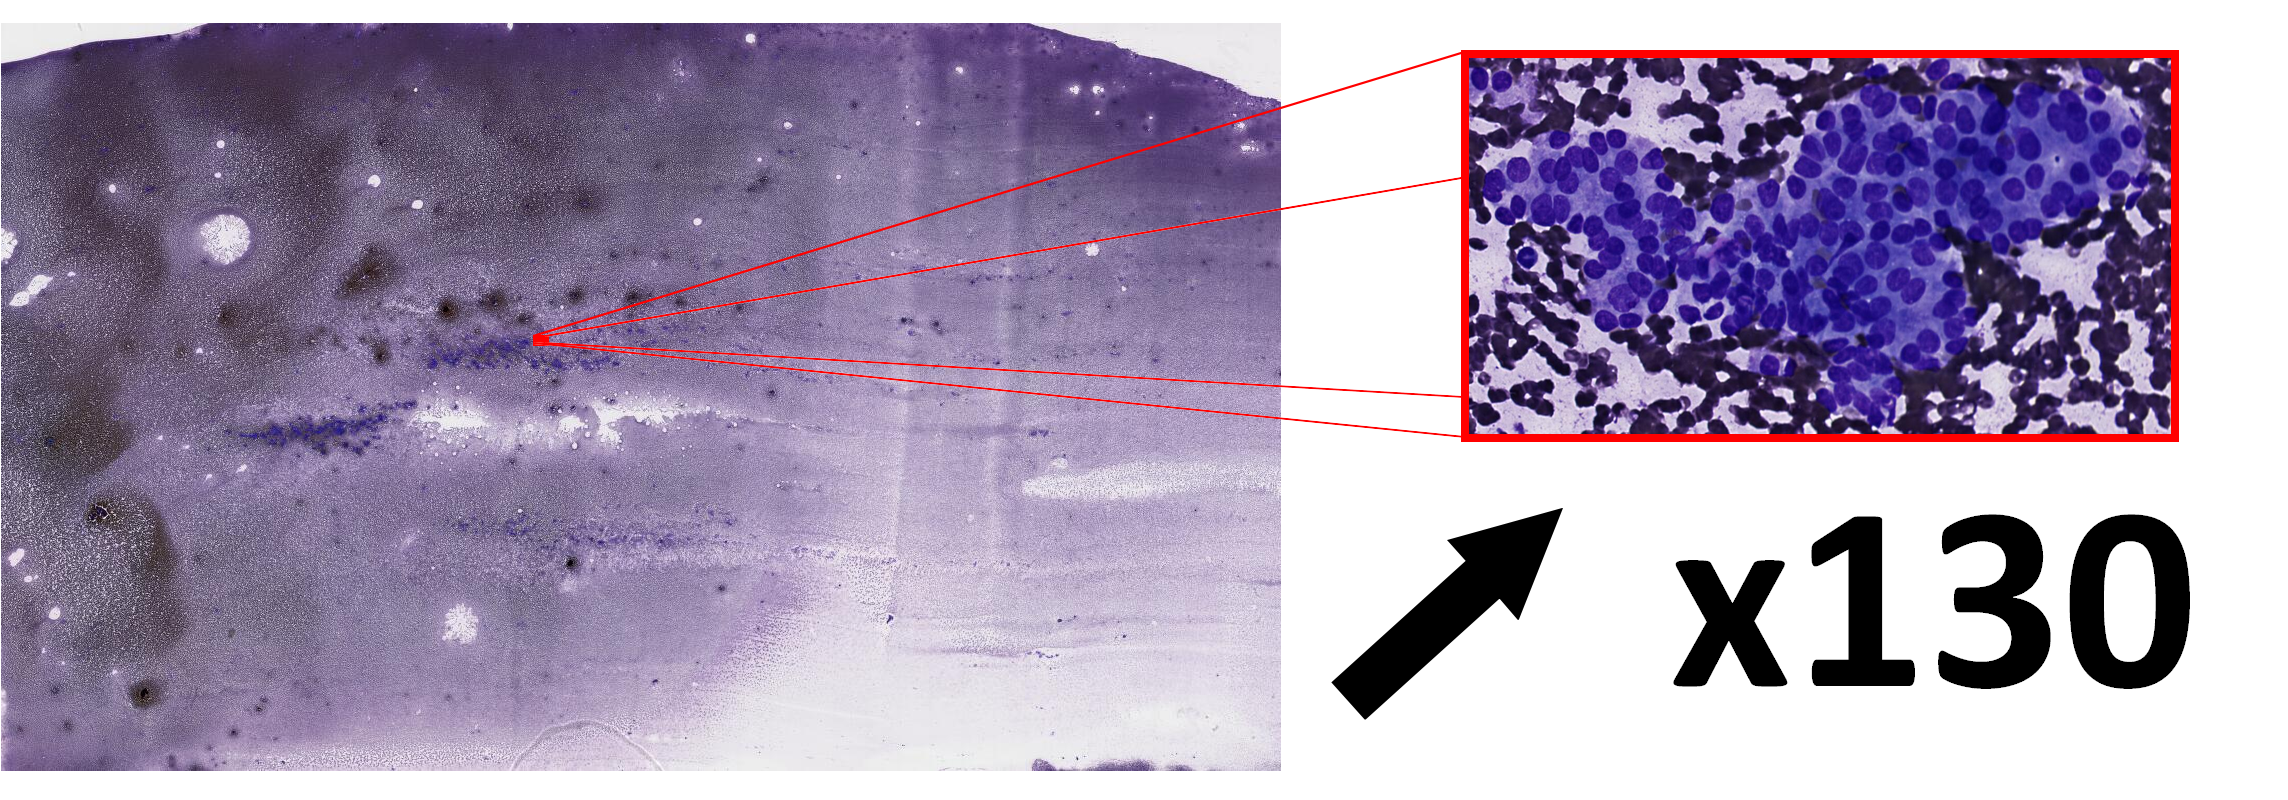
\includegraphics[scale=0.6]{images/whole-slide-dim.png}
\caption{To the left, a microscope slide smeared with thyroid cell samples (15 gigapixels). To the right, an object of interest: a proliferative architectural pattern.}
\end{figure}

\begin{itemize}
\item Thanks to modern technologies, microscope slides are often digitized to be further analysed on computers. But \textbf{slides are huge}: $\sim$ 100K $\times$ 100K pixels typically  ($\sim 10^{10}$ pixel$^2$)
\item Due to the lack of proper tool, those slides are \textbf{usually analysed manually} ! 
\item \textbf{Machine learning and image processing} could provide a great alternative to a pure-human approach.
\end{itemize}		

\begin{center}
\large
$\Rightarrow$ Those problems can be expressed as problems of \textbf{object detection and classification}.
\end{center}

\end{block}

~~

\begin{block} {SLDC framework}
\textit{SLDC} is an \textbf{open-source Python framework} created for accelerating development of large image analysis workflows which can be expressed as problems of object detection and classification.

~

\textbf{How ?}
\begin{itemize}

\item It \textbf{encapsulates problem-independent logic} (parallelism, memory limitation due to large images handling,…)

\item It provides a \textbf{concise way of declaring problem dependant components} (segmentation, object classification,…)

\end{itemize}

~~

\begin{alertblock}{Features}
\begin{itemize}
\item \textbf{Tile-based}: images are splitted into tiles which are loaded one after another into memory. A full image is never loaded into memory at once.
\item \textbf{Parallel}: available at several levels (tiles, objects, images,...).
\item \textbf{Talkative}: a customizable logging system provides a real-time rich feedback about the execution.
\item \textbf{Integrable}: thanks to Python, integration with other libraries such as scikit-learn (ML), open-cv (IP), PyCuda (GPU),... is effortless.
\item \textbf{Convenient}: builder components provide an easy way of constructing complex workflows.
\end{itemize}
\end{alertblock}

~~ 

\begin{alertblock}{How SLDC works}
Given an input image, the framework produces a set of polygons and classification labels representing the objects and their labels. In order to do so, it executes the following steps: 

~

\begin{itemize}
\item \textbf{S}egment $\mathcal{S}$: a segmentation procedure is applied on the input image (top-left) and produces a binary mask (top-right) locating the objects of interest in the image.
\item \textbf{L}ocate $\mathcal{L}$: polygons representing the objects found in the image are extracted from the binary mask.
\item \textbf{D}ispatch $\mathcal{D}$: polygons are dispatched to their most appropriate classifier using some dispatching rules $r$. 
\item \textbf{C}lassify $\mathcal{T}_i$: a classifier produces a classification for the polygons/objects it is passed.
\end{itemize}

~

All problem-independent concerns being encapsulated by the framework, developers only have to define the segmentation $\mathcal{S}$, the dispatching rules $r$ and the classifiers $\mathcal{T}_i$.

~

\begin{figure}
\center
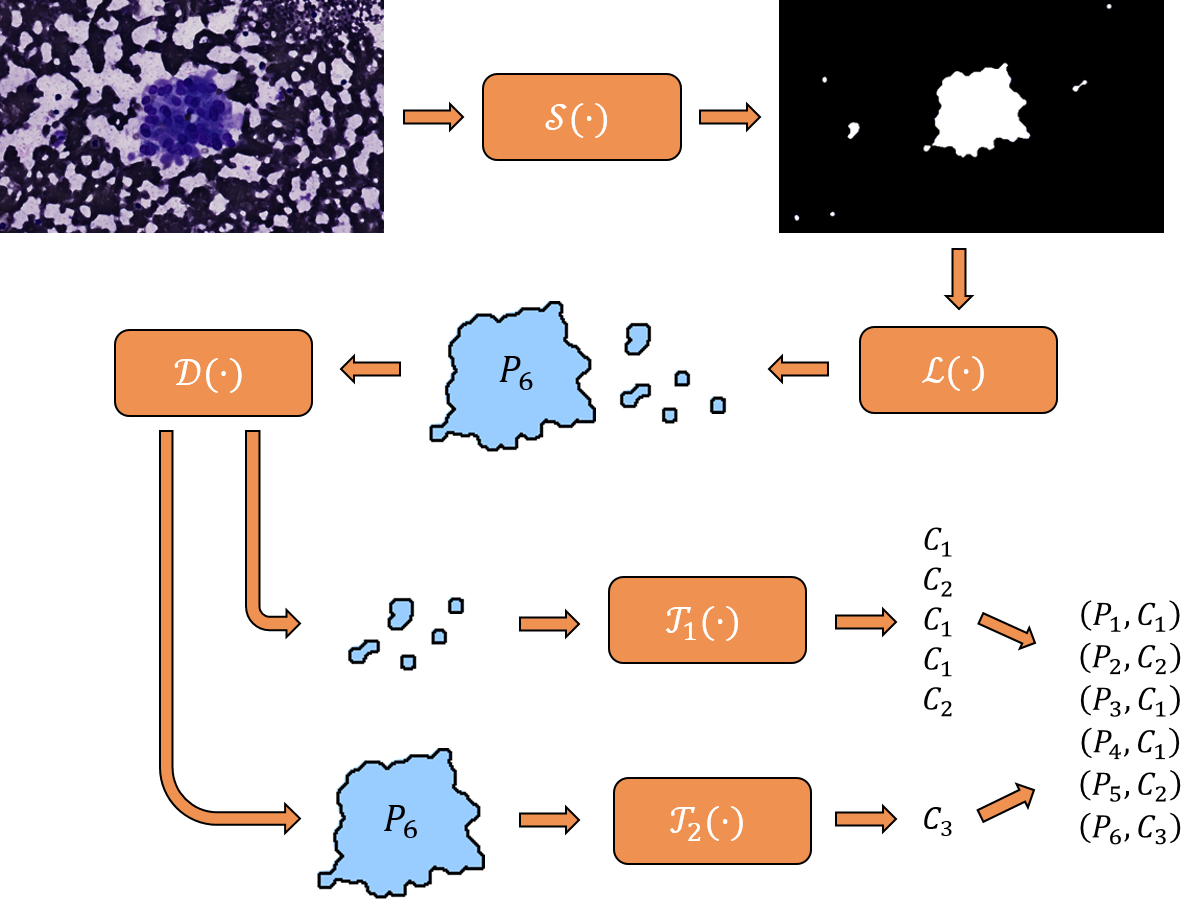
\includegraphics[scale=1.3]{images/workflow_illustration.png}
\end{figure}

\end{alertblock}
\end{block}

\column{.45\paperwidth}

\begin{block}{SLDC at work: thyroid nodule malignancy diagnosis}
To diagnose thyroid cancer, cytopathologists screen microscope slides smeared with thyroid nodule cell samples. The illness is diagnosed when two types of objects are found on those slides: 

\begin{figure}
	\subfigure[Cells with inclusion]{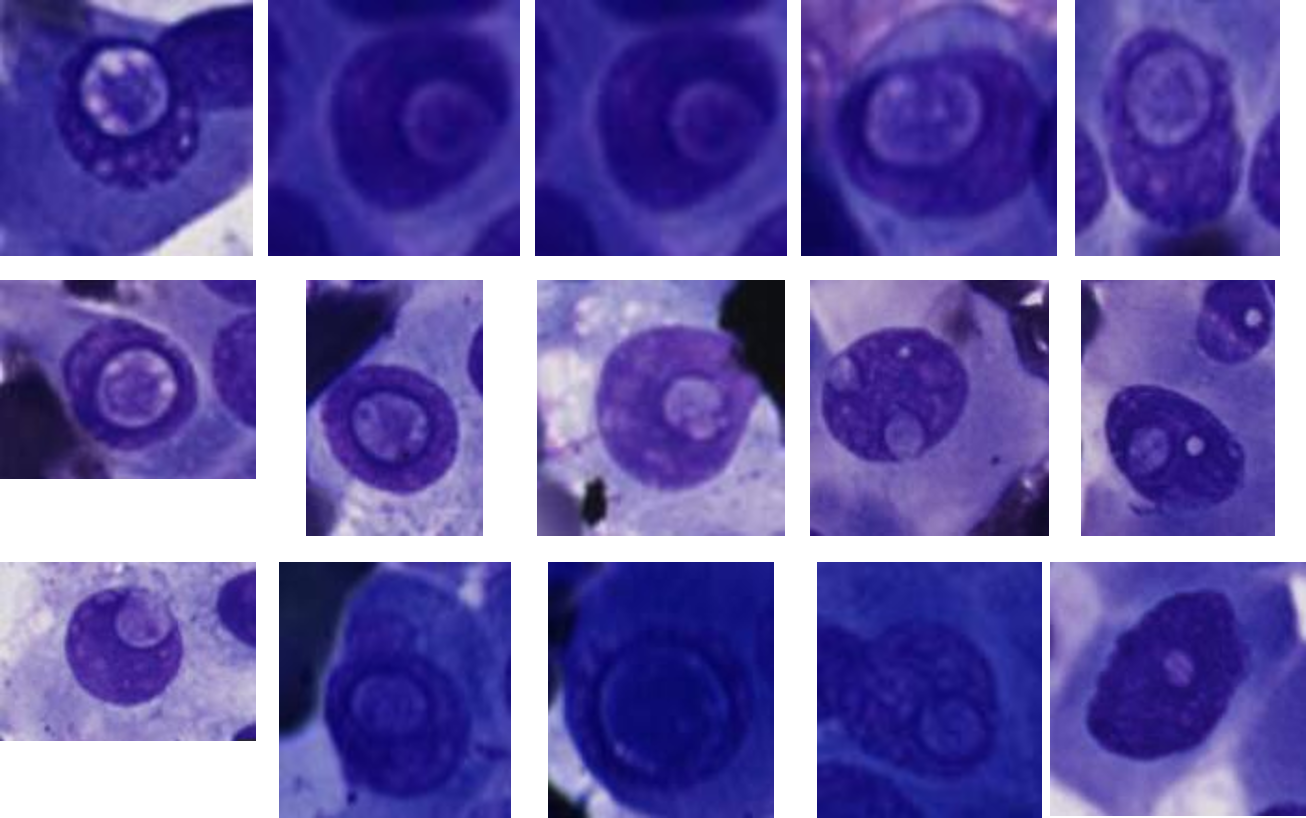
\includegraphics[scale=0.32]{images/all_incl.png}}
	\hspace{1cm}
	\subfigure[Proliferative patterns]{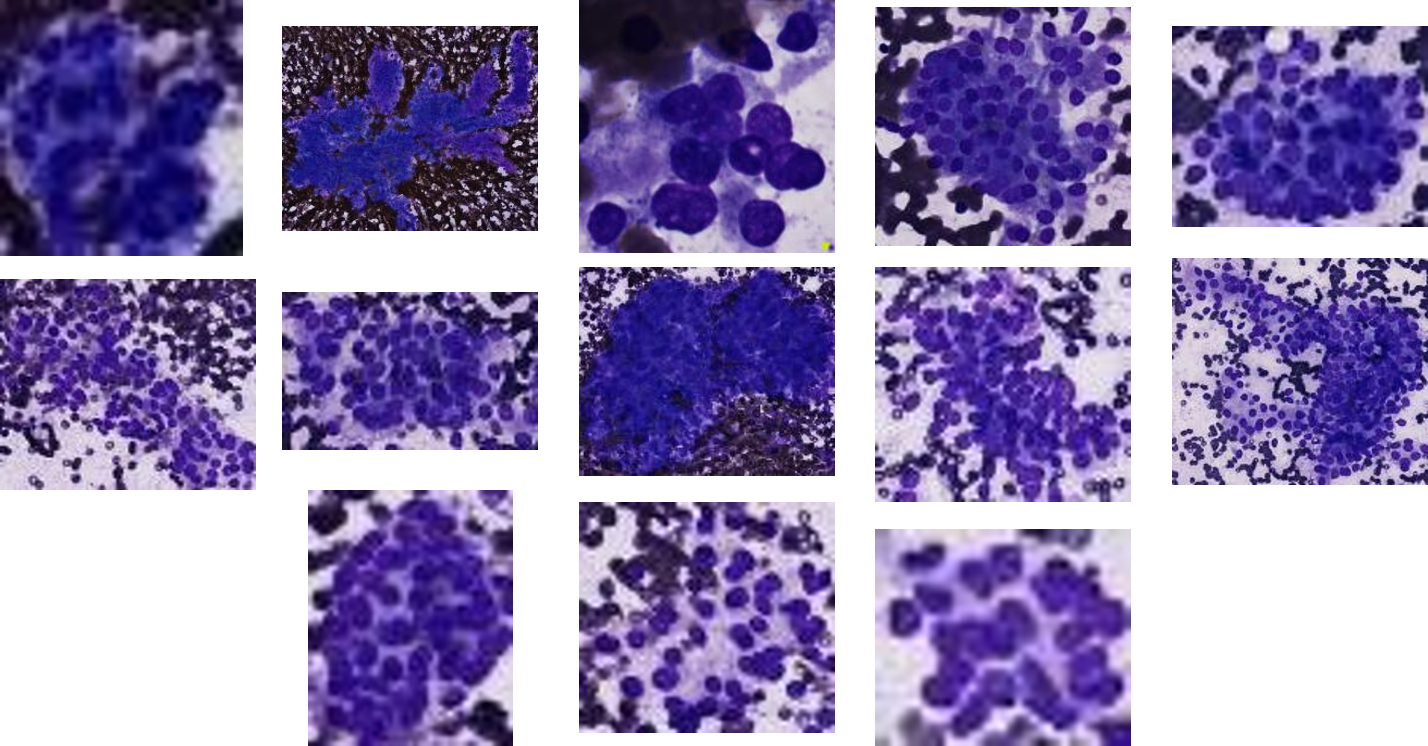
\includegraphics[scale=0.345]{images/all_prolif.png}}
\end{figure}
\end{block}

\begin{exampleblock}{Data}

The dataset is stored on the Cytomine \cite{maree2016collaborative} web platform. In consists in:

\begin{itemize}
	\item \textbf{84 images} with size ranging from 4 to 18 gigapixels
	\item \textbf{68 annotated images} 
	\item \textbf{5921 labelled annotations} made by cytopathologists from ULB (Team of Pr. Isabelle Salmon, Dept. of Pathology)
\end{itemize}

\begin{figure}
\center
\subfigure[Annot. per group]{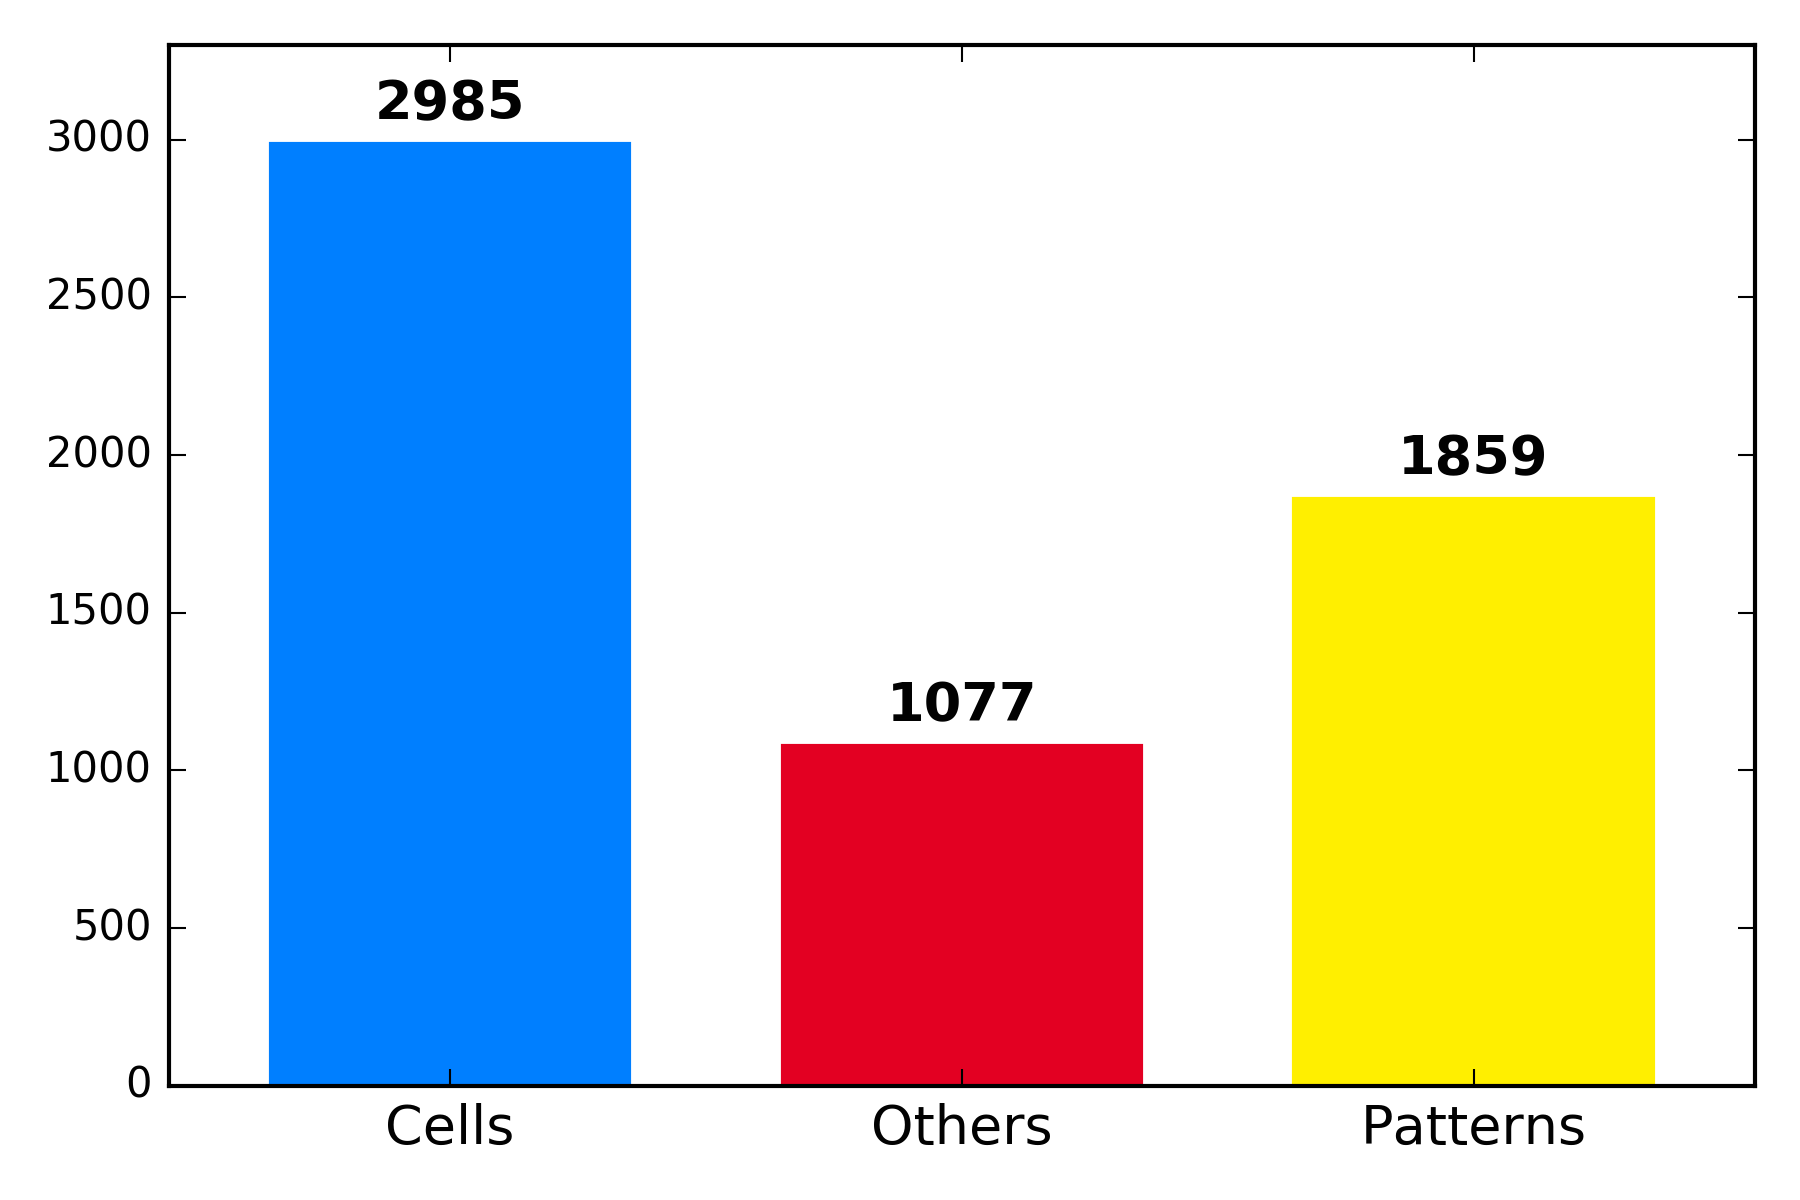
\includegraphics[scale=0.65]{images/counts_all_grouped.png}}
\subfigure[Pattern annot. per group]{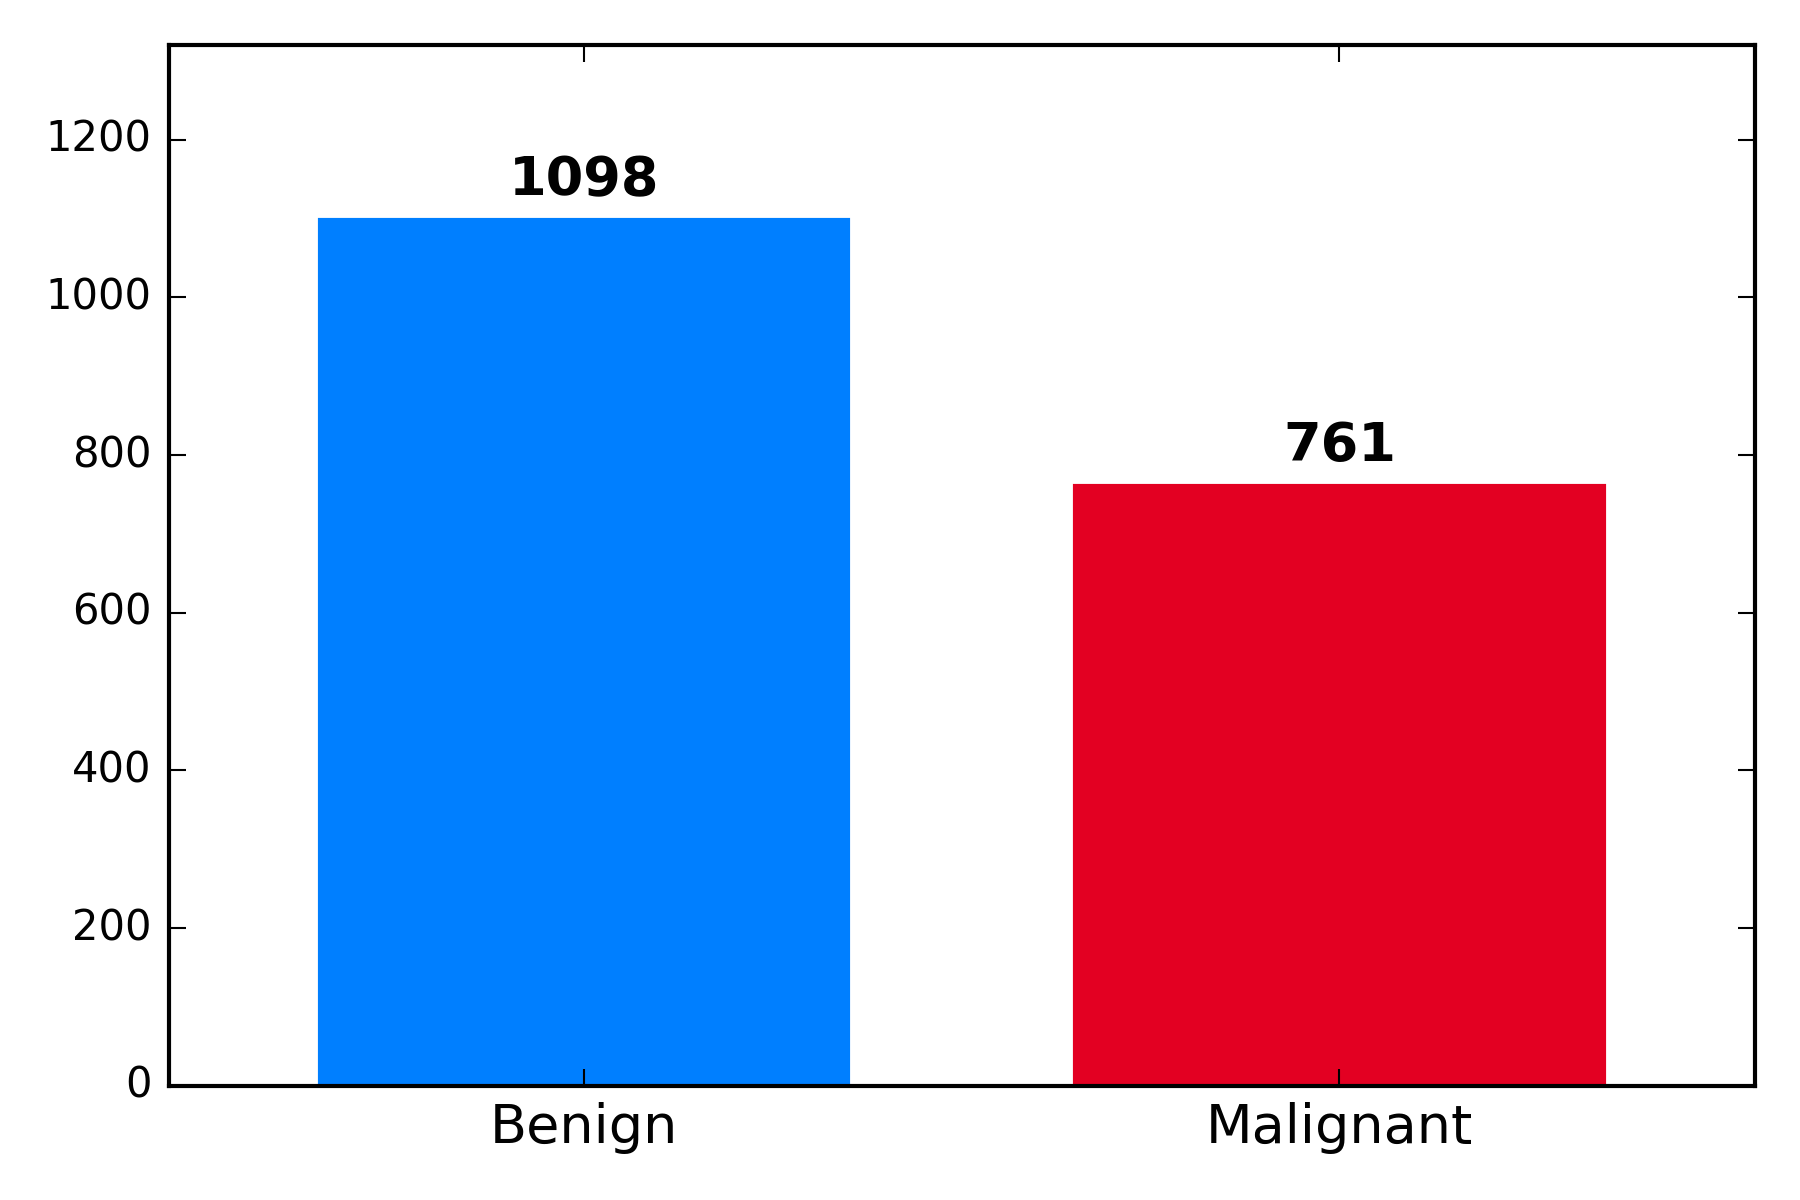
\includegraphics[scale=0.65]{images/counts_patterns_grouped.png}}
\subfigure[Cell annot. per group]{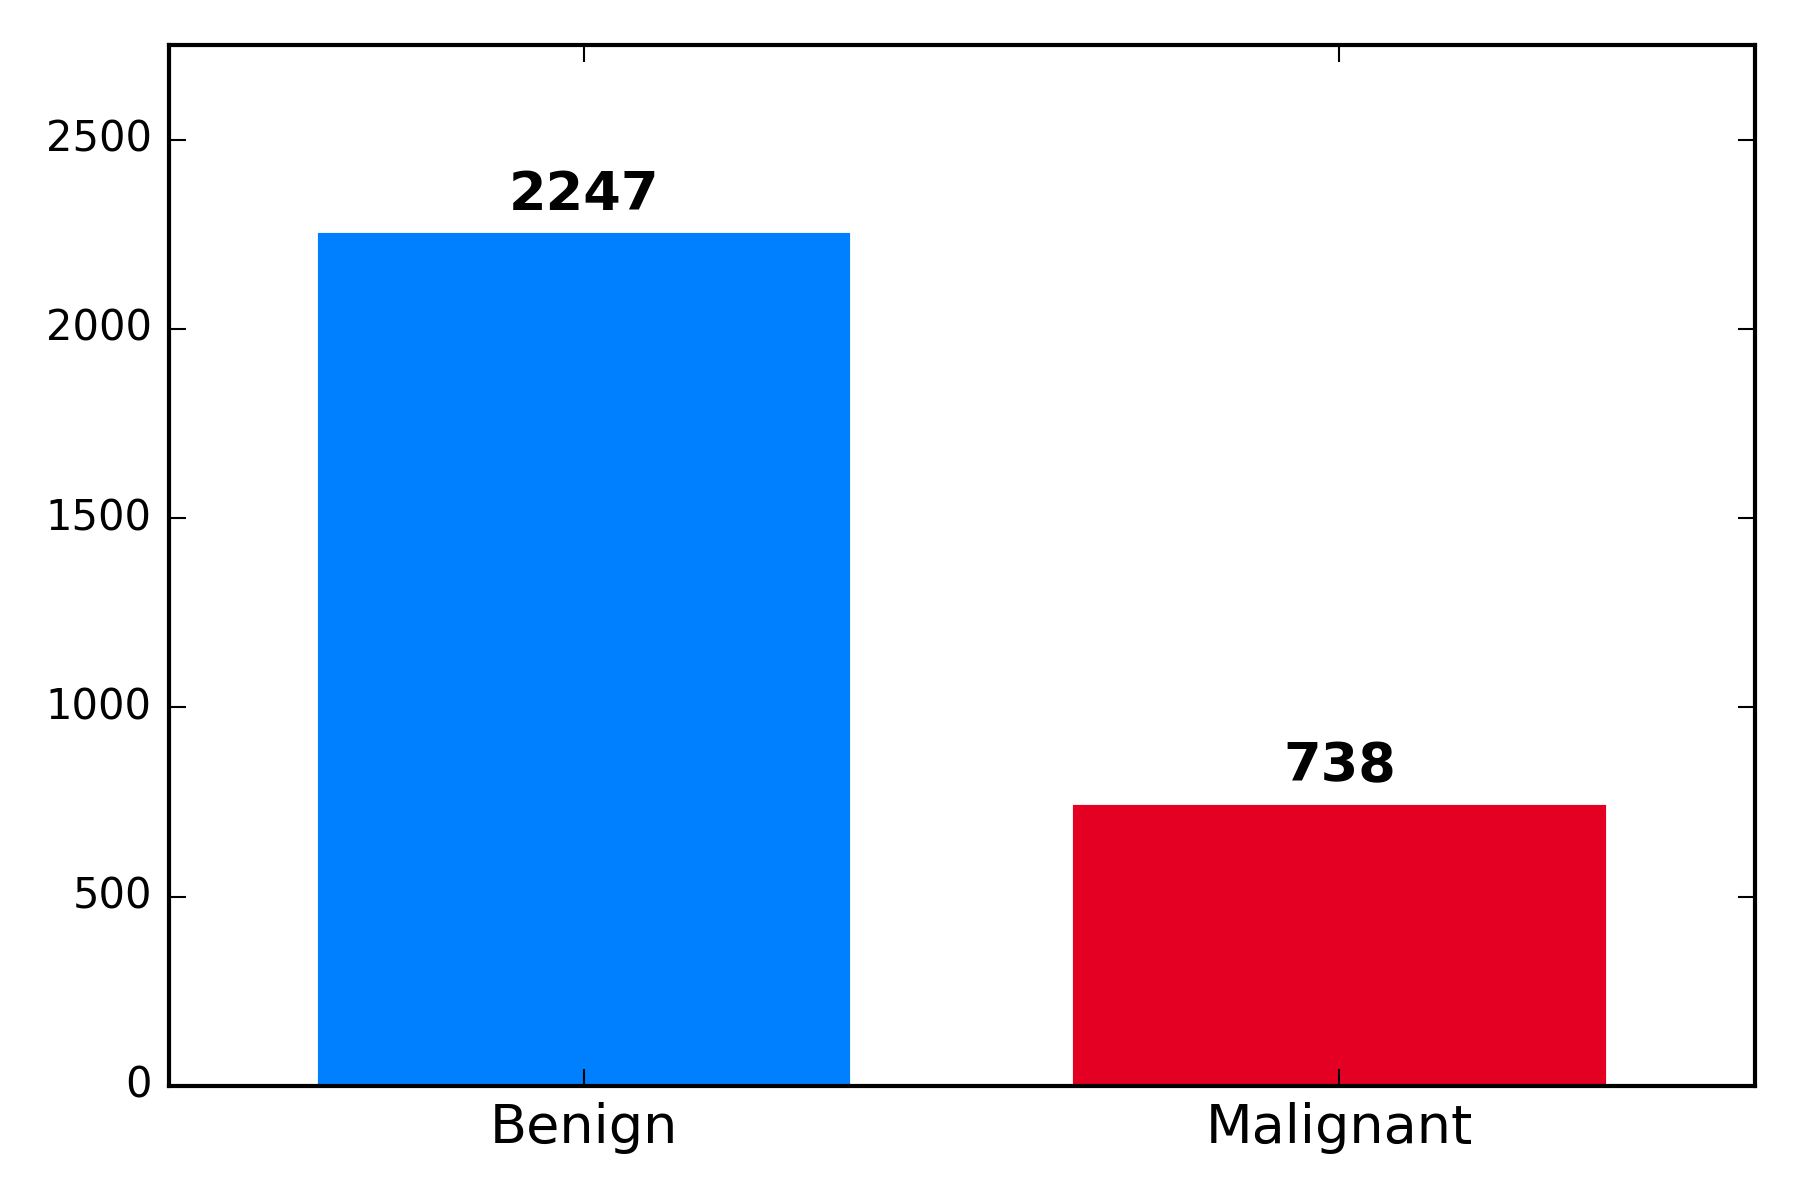
\includegraphics[scale=0.65]{images/counts_cells_grouped.png}}\\
\subfigure[Annot. per term]{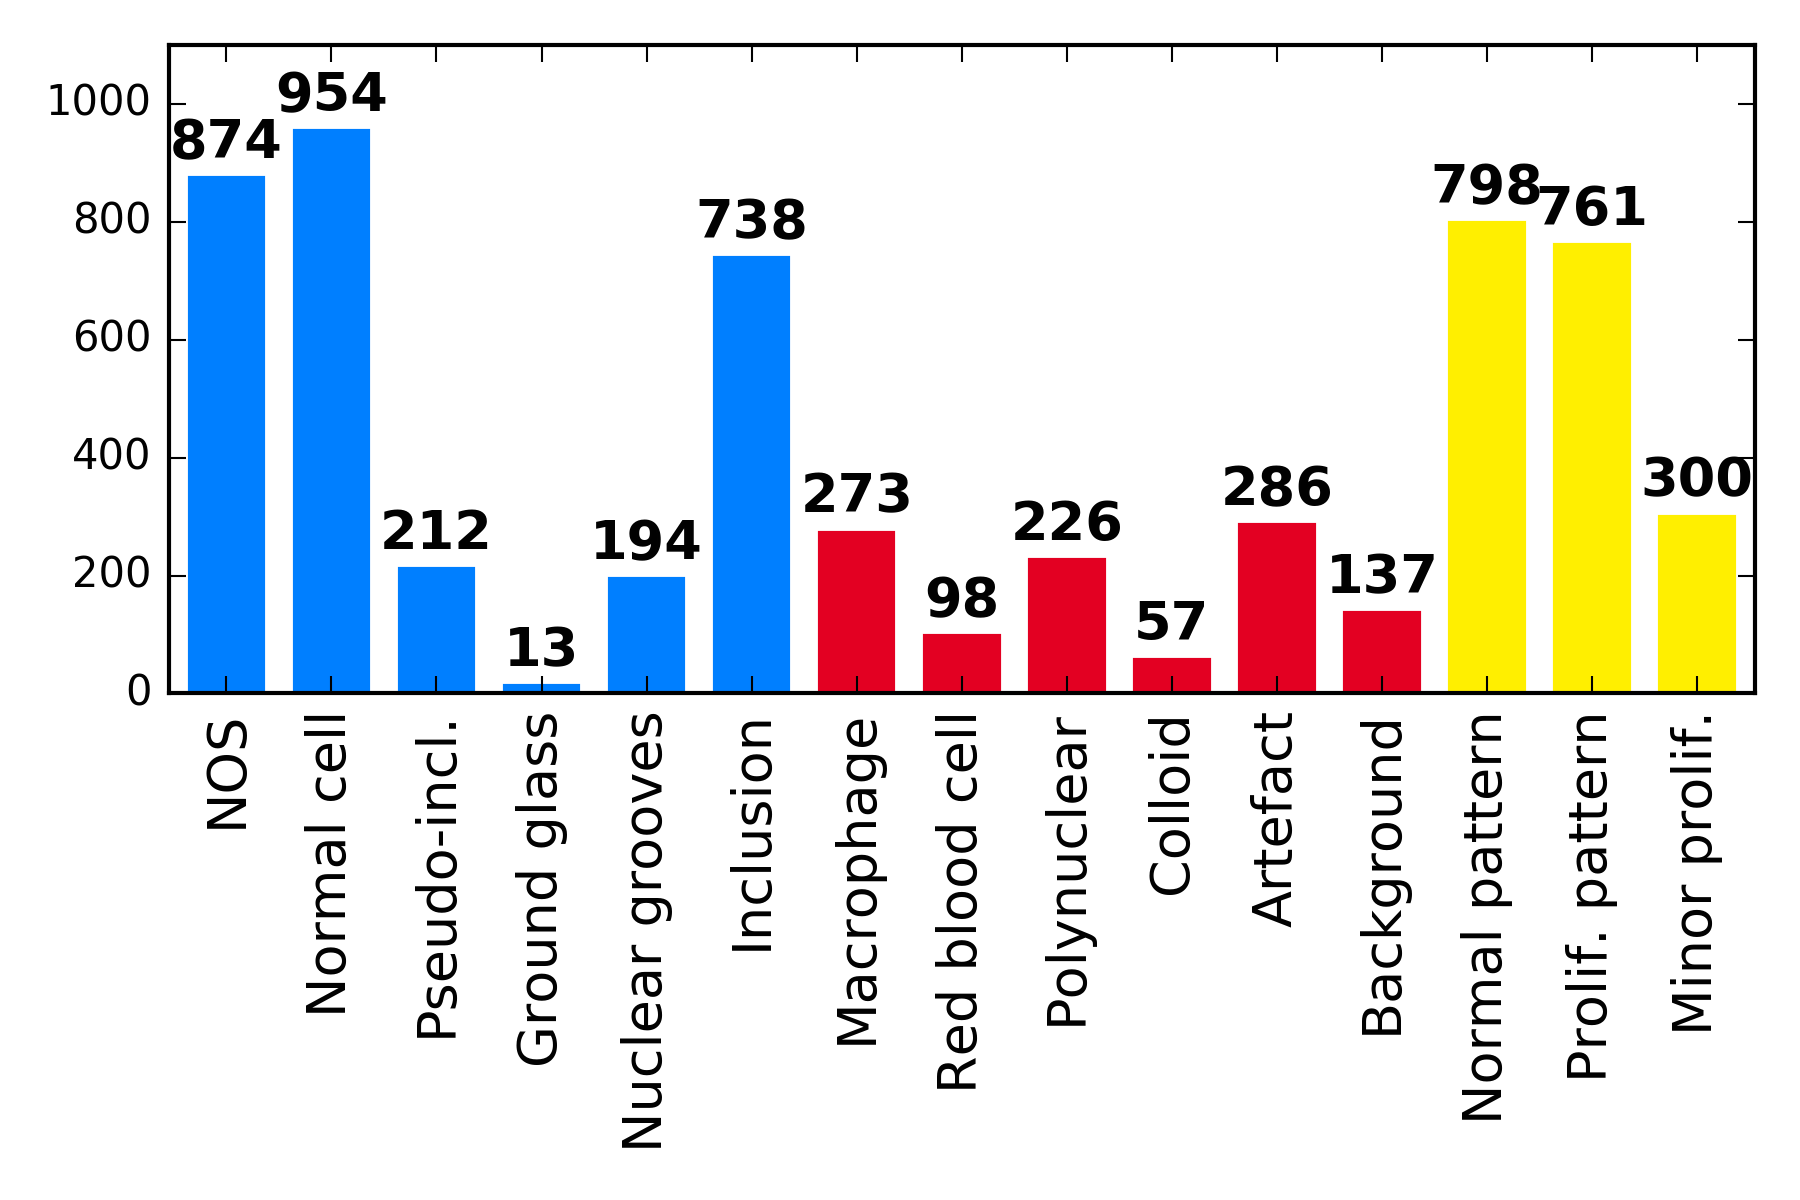
\includegraphics[scale=0.65]{images/counts_all.png}}
\subfigure[Pattern annot. per term]{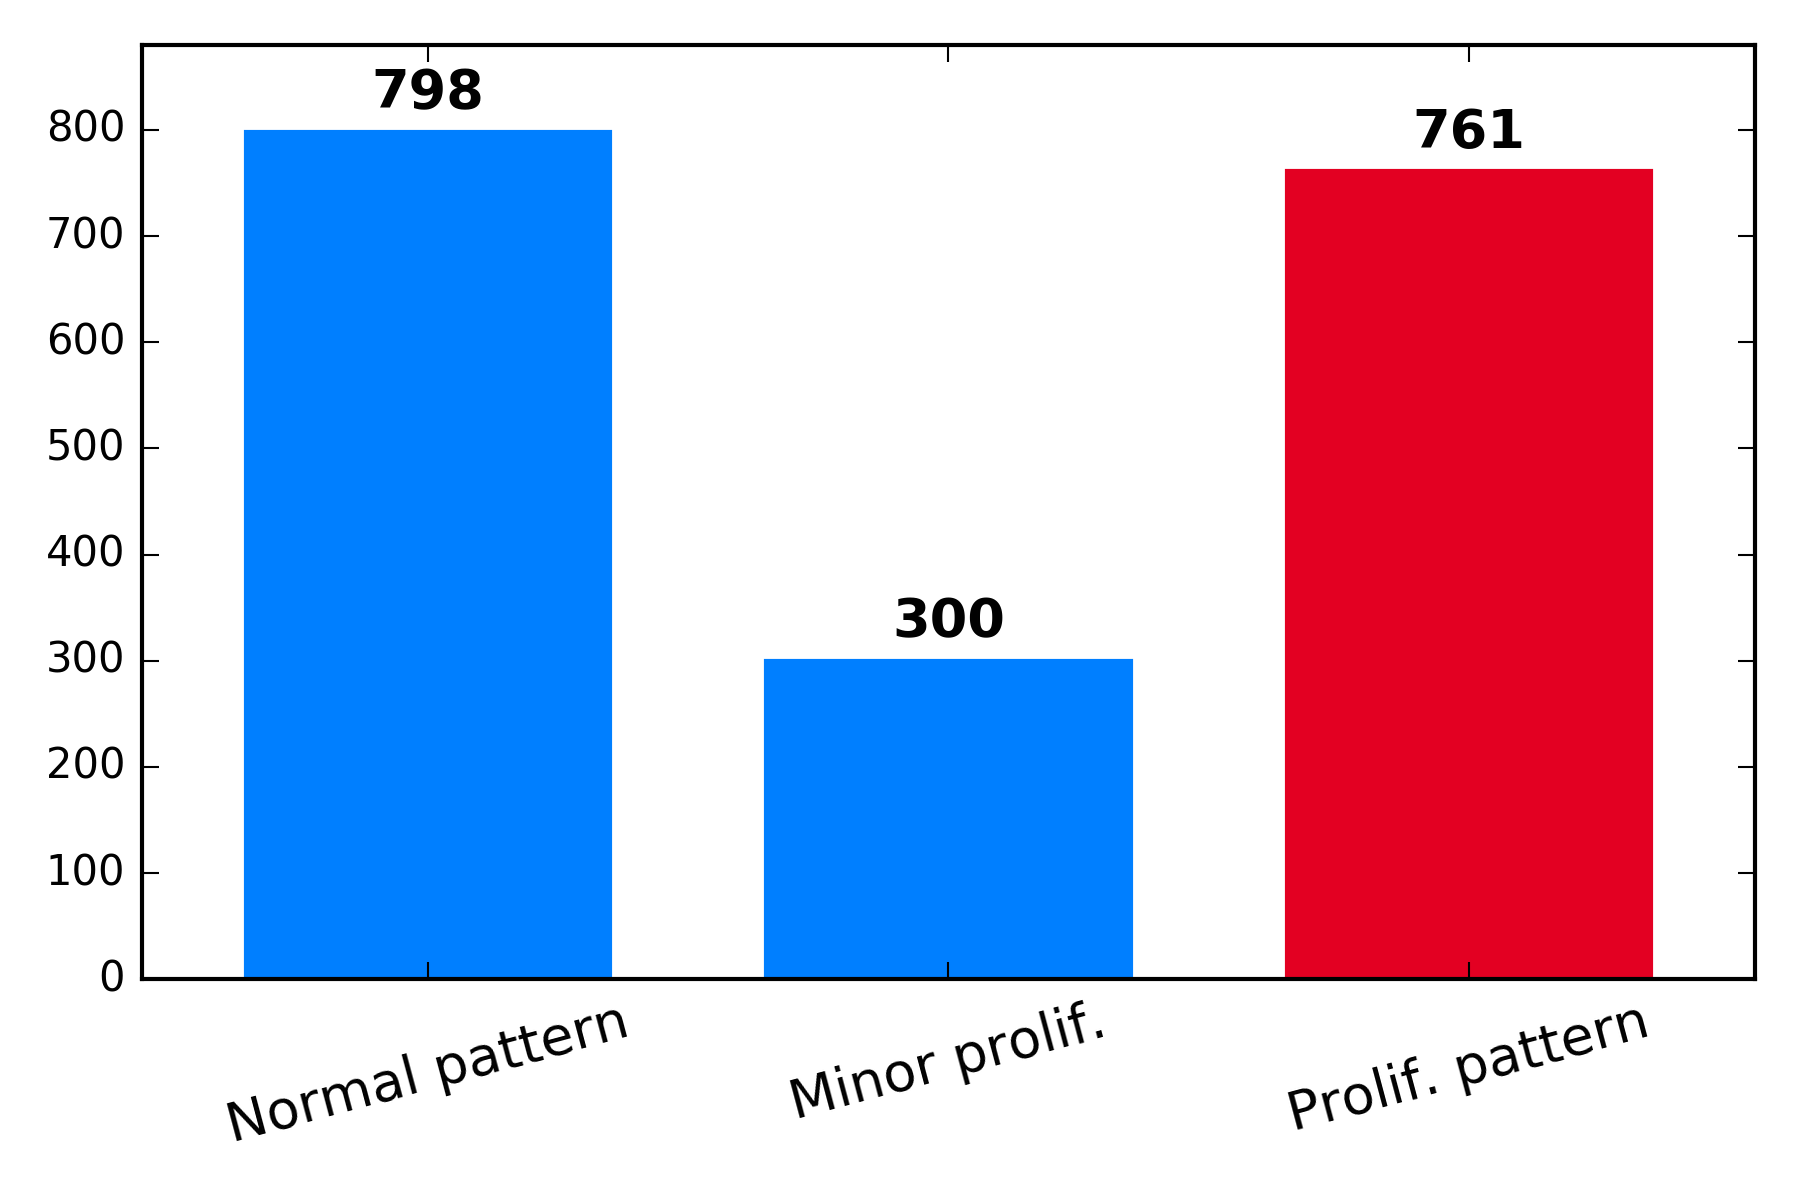
\includegraphics[scale=0.65]{images/counts_patterns.png}}
\subfigure[Cell annot. per term]{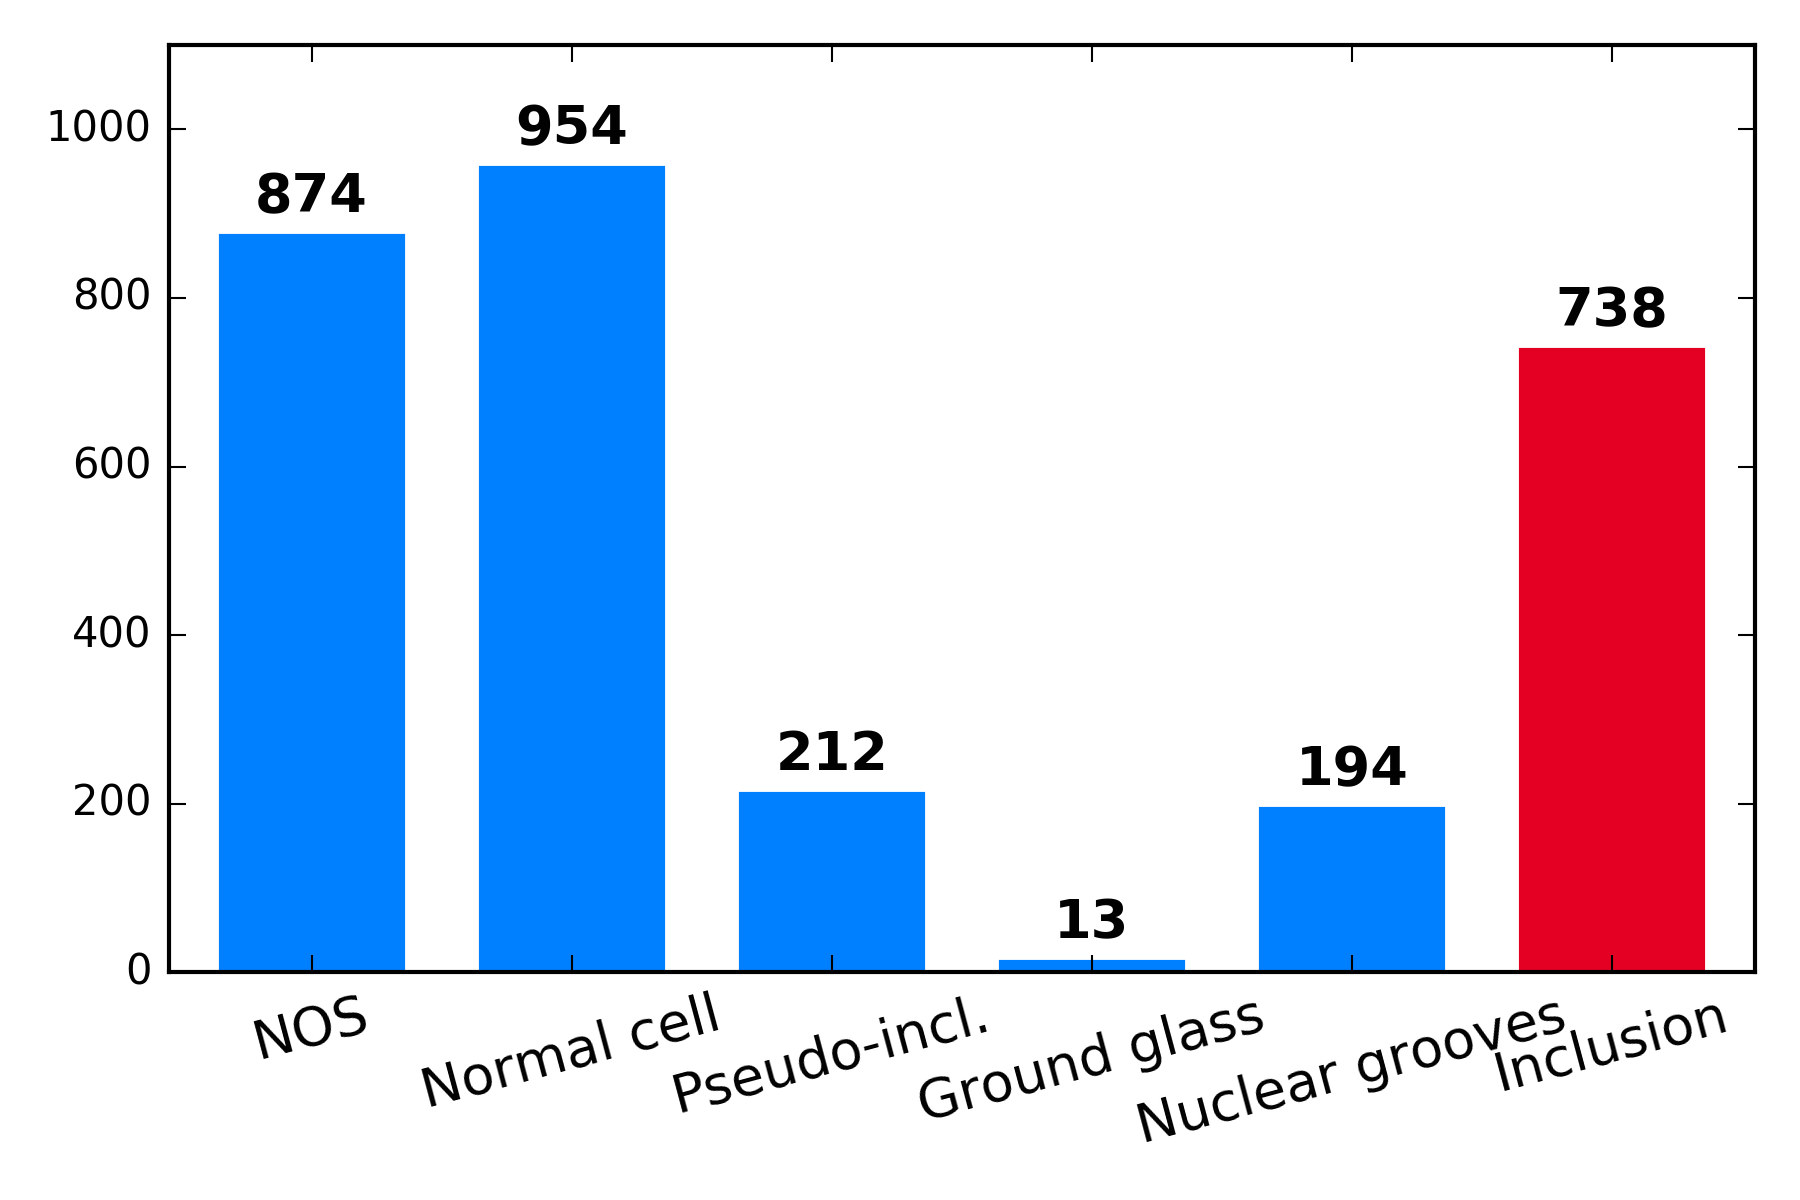
\includegraphics[scale=0.65]{images/counts_cells.png}} \\
\subfigure[Normal patterns (benign)]{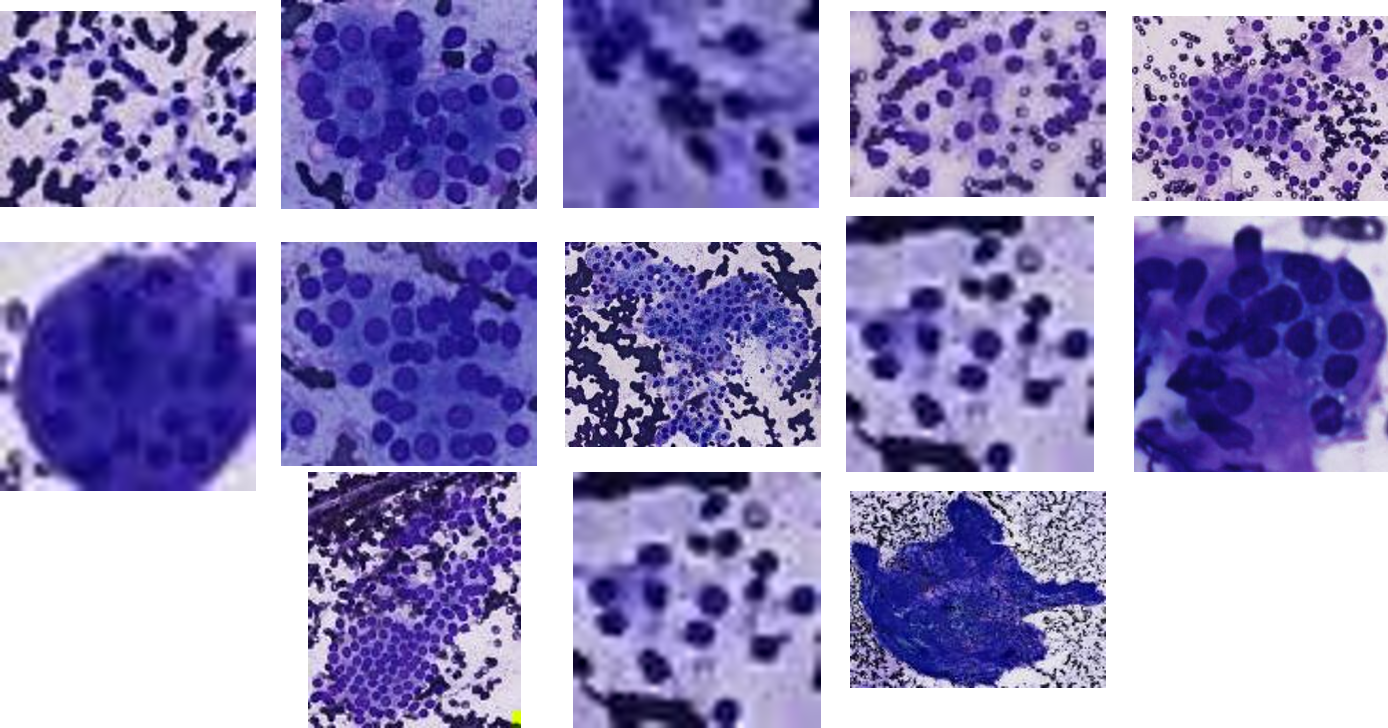
\includegraphics[scale=0.19]{images/all_norm_patterns.png}}
\subfigure[Proliferative (malignant)]{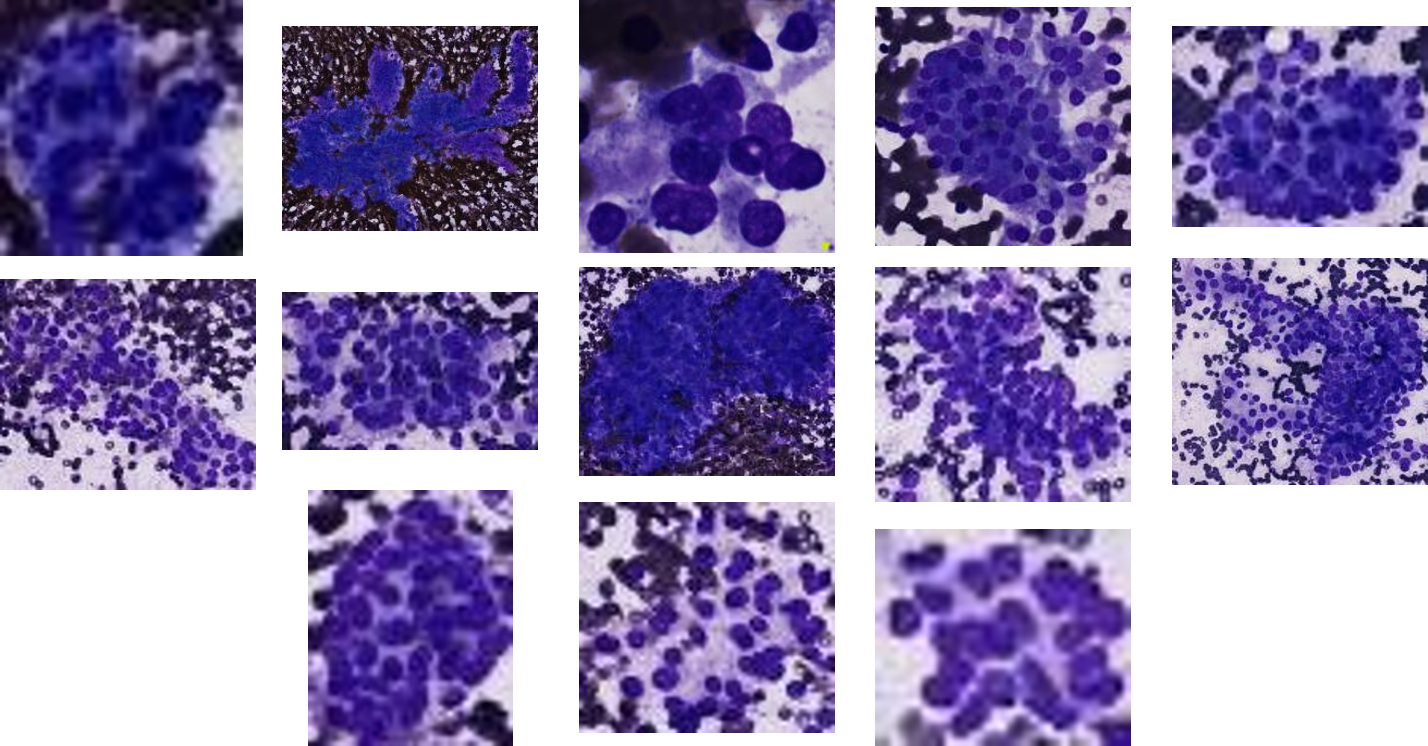
\includegraphics[scale=0.19]{images/all_prolif.png}}
\subfigure[Normal cells (benign)]{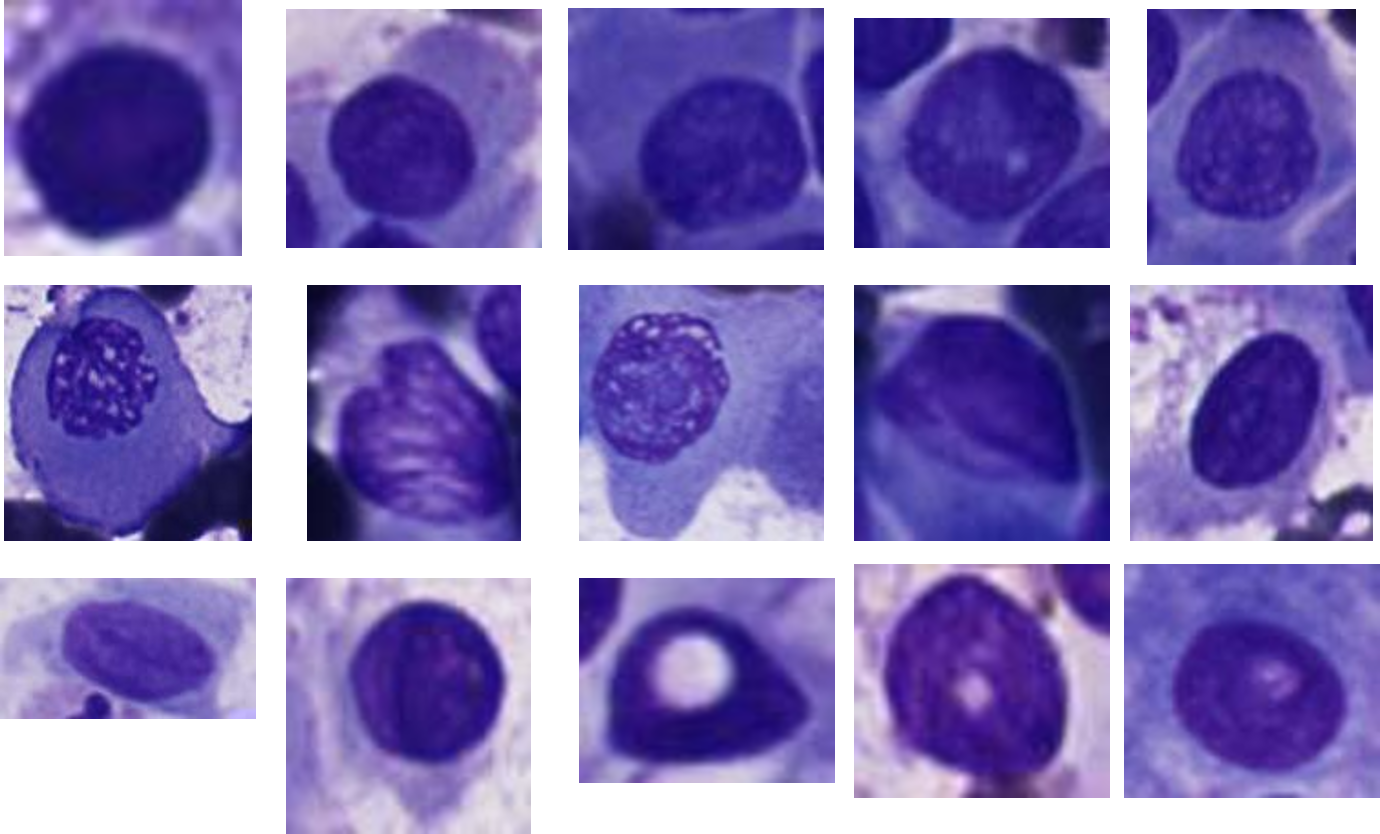
\includegraphics[scale=0.16]{images/all_norm_cells.png}}
\subfigure[Cells with incl. (malignant)]{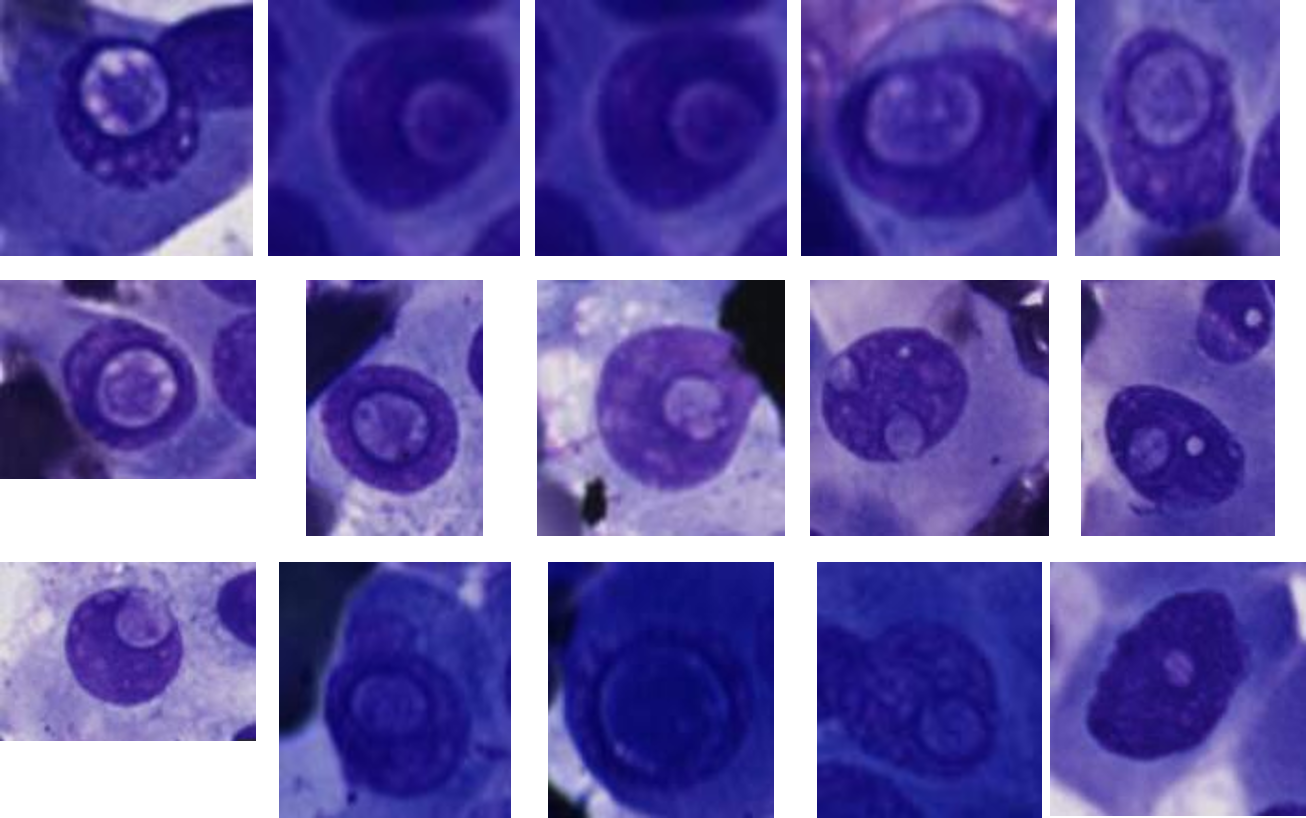
\includegraphics[scale=0.16]{images/all_incl.png}}
\end{figure}
	
\end{exampleblock}

\begin{exampleblock}{Workflow}
Two passes are performed on the images. The first consists in extracting standalone cells and architectural patterns. The second consists in extract cells which are contained in the detected patterns. 

\begin{figure}
	\center
	\subfigure[First pass workflow]{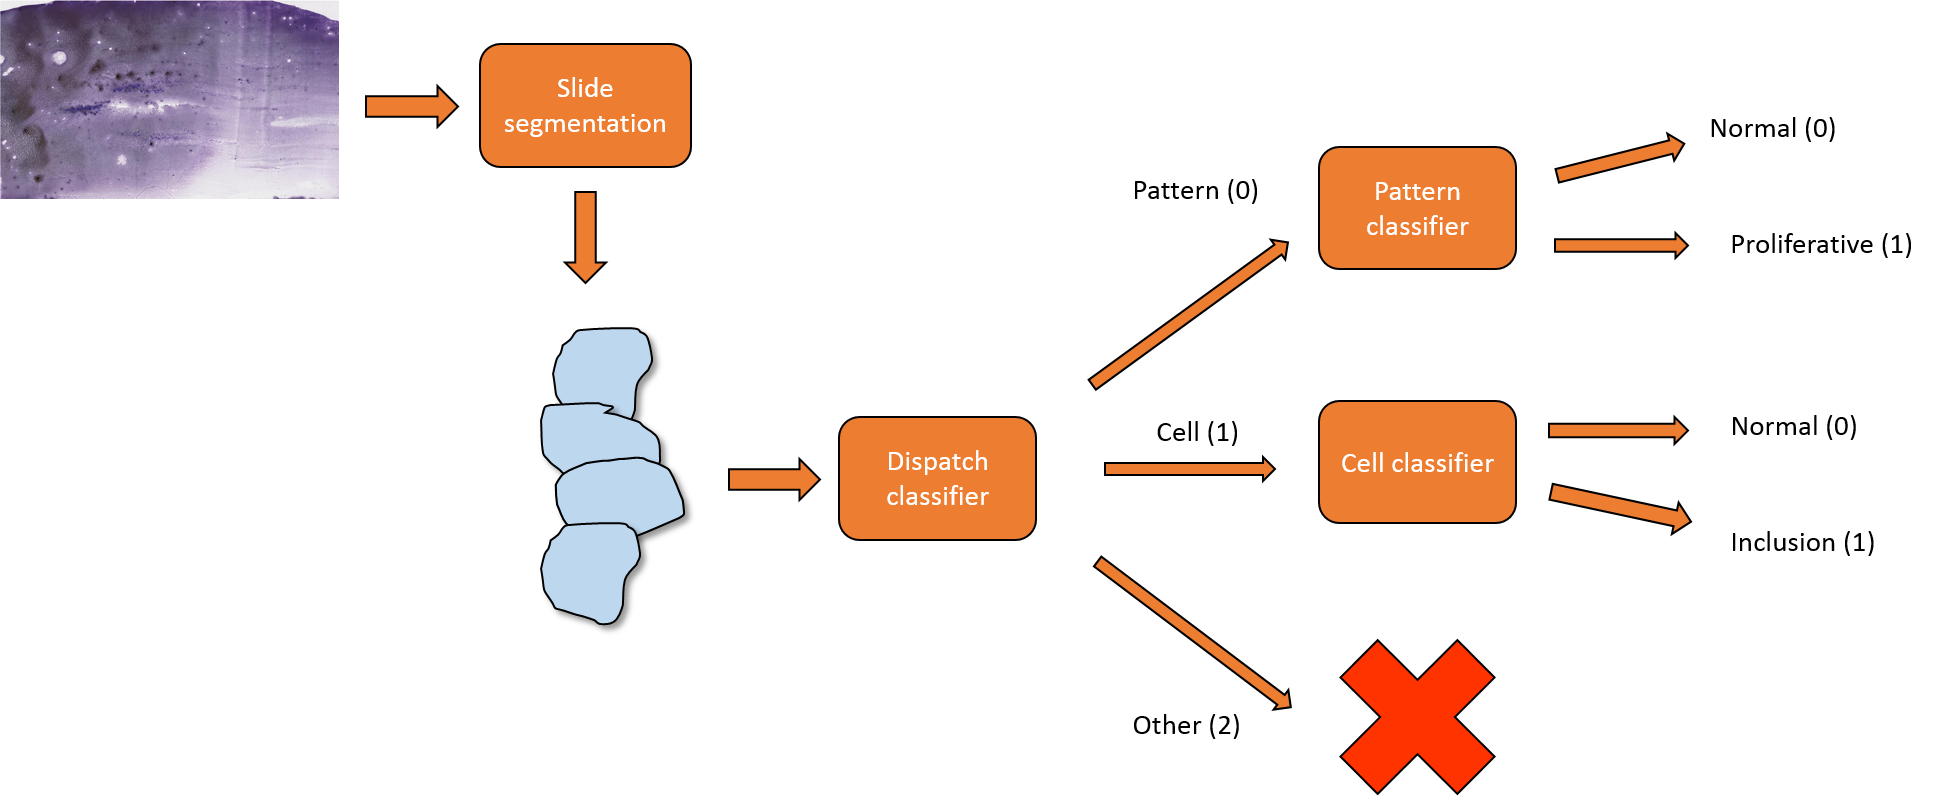
\includegraphics[scale=0.55]{images/thyroid_workflow_1.png}}
	\subfigure[Second pass workflow]{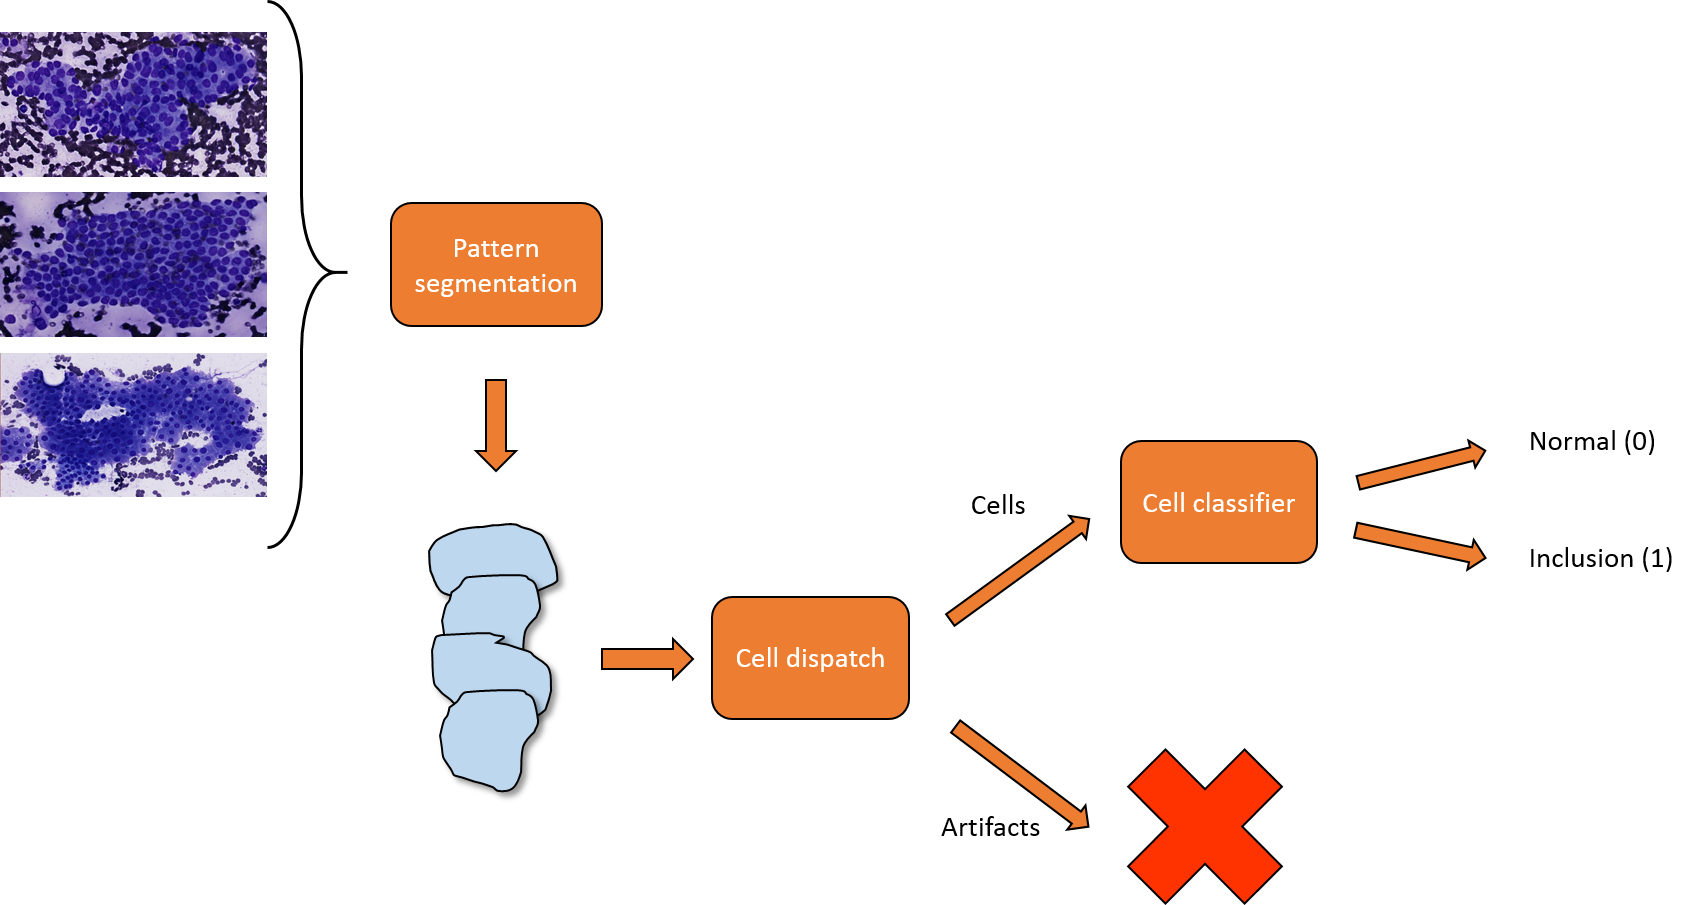
\includegraphics[scale=0.65]{images/thyroid_workflow_2.png}}
\end{figure}

\end{exampleblock}

\begin{exampleblock}{Classification}
Classification is performed based on the detected object's crop image using \textbf{random subwindows and extremely randomized trees} \cite{Maree201617}.
\end{exampleblock}

\begin{exampleblock}{Results}

	\begin{columns}
		\begin{column}{0.48\linewidth}
			\begin{figure}
				\center
				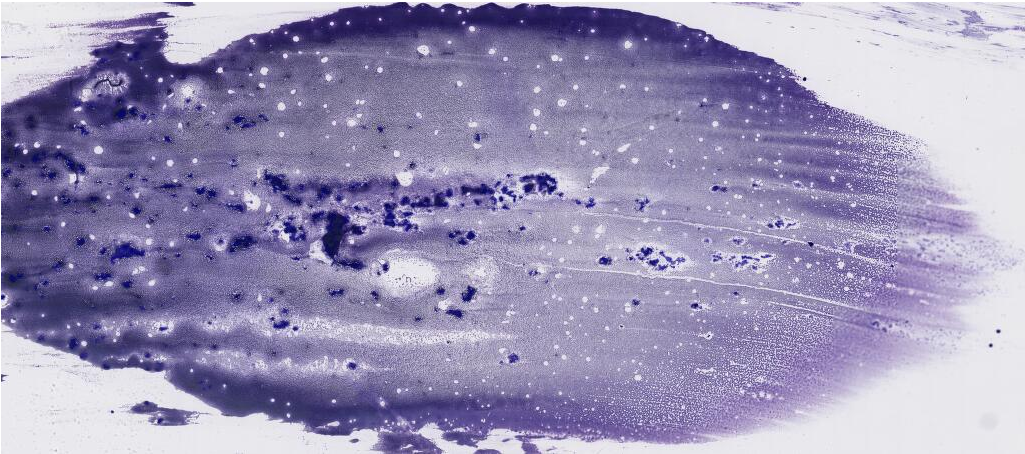
\includegraphics[scale=0.6]{images/728725.png}
			\end{figure}
			
			\begin{tabular}{rl}			
				& \\			
				Size: & 131072 $\times$ 57856\\	
				Objects found: & \textbf{20046} \\
				Cells found: & 18966 \\
				Patterns found: & 1080 \\
				& \\
				Time (1st pass): & \textbf{7 min 30 sec} \\
				Time (2nd pass): & 1 h 10 min  \\
				Peak memory: & 138 Go \\
			\end{tabular}
		\end{column}

		\begin{column}{0.48\linewidth}
			\begin{figure}
				\center
				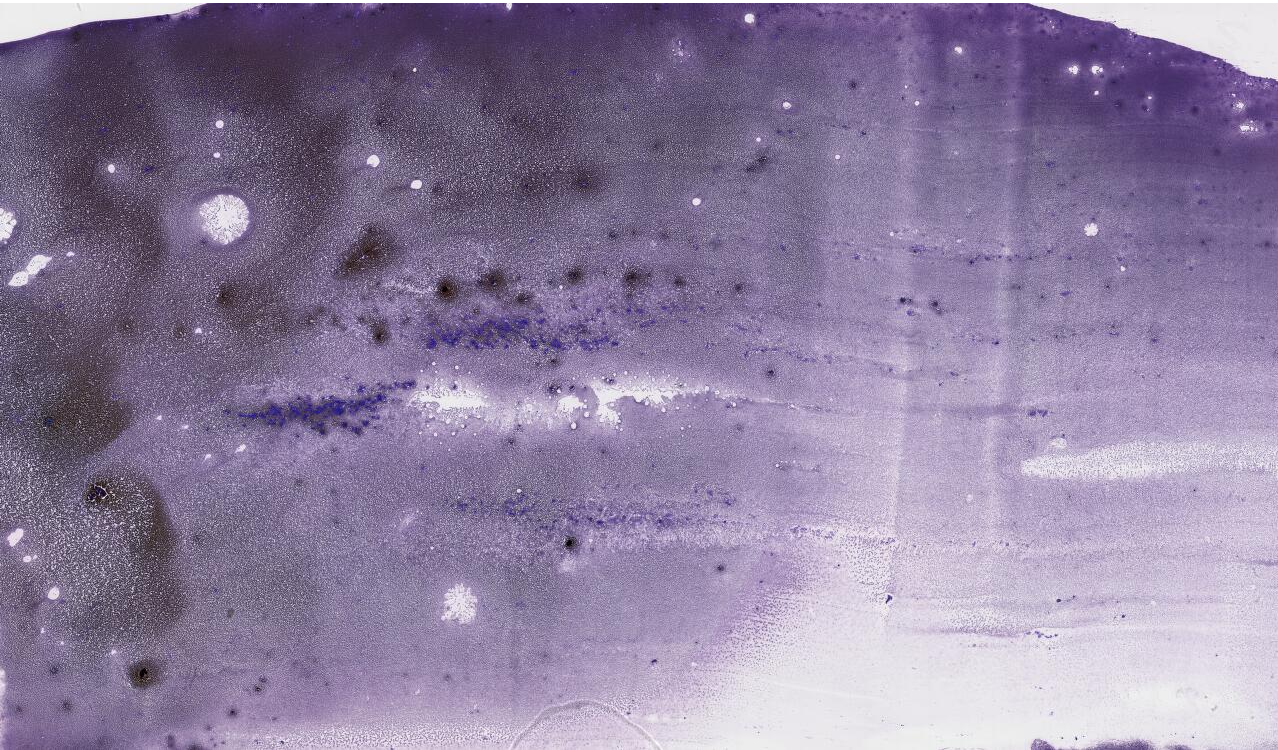
\includegraphics[scale=0.35]{images/716528.png}
			\end{figure}
			
			\begin{tabular}{rl}
				& \\
				Size: & 163840 $\times$ 95744 \\
				Objects found: & \textbf{79063} \\
				Cells found: & 72740 \\
				Patterns found: & 6323 \\
				& \\
				Time (1st pass): & \textbf{18 min 20 sec} \\
				Time (2nd pass): & 4 h 50 min  \\
				Peak memory: & 178 Go \\
			\end{tabular}
		\end{column}
	\end{columns}
\end{exampleblock}
\vfill

\begin{alertblock}{Conclusion}
\begin{enumerate}
	\item The framework is production ready, feel free to use it! 
	\item The thyroid workflow can still be improved (classifiers and segmentations)
\end{enumerate}
\end{alertblock}
\begin{block}{Bibliography}
\printbibliography
\end{block}

\end{columns}
\end{frame}
\end{document}
